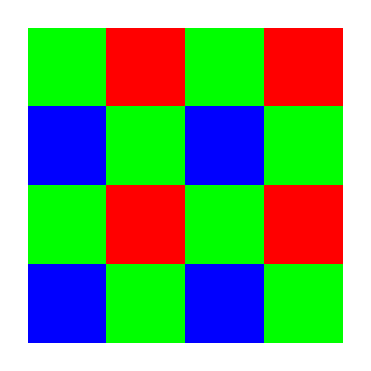
\begin{tikzpicture}

% Loop to draw the squares
\foreach \i in {0,1,2,3} {
    \foreach \j in {0,1,2,3} {
        \pgfmathtruncatemacro{\row}{mod(\i, 2)}
        \pgfmathtruncatemacro{\col}{mod(\j, 2)}
        
        % Choose color based on position
        \ifnum \row=0
            \ifnum \col=0
                \def\fillcolor{blue}
            \else
                \def\fillcolor{green}
            \fi
        \else
            \ifnum \col=0
                \def\fillcolor{green}
            \else
                \def\fillcolor{red}
            \fi
        \fi

        % Draw the square
        \fill[\fillcolor] (\i,\j) rectangle ++(1,1);
    }
}

\end{tikzpicture}